% !TeX spellcheck = <none>

\chapter{Background}

Fiber-reinforced composite materials (FRC) are seeing a widespread use in a large number of applications ranging from aerospace systems over renewable energy production to automotive parts \cite{park2011interface} \cite{HighPerformanceTextiles}. 
These composite materials generally provide high specific strength and improved stiffness compared to other materials \cite{GeneralizedContinuumMechanics}. 
Through the combination of different materials, desirable mechanical properties like low weight with high stiffness can be achieved that would be hard or near impossible to recreate with single compound materials \cite{AdvancesDamageMechanics}. 
The attributes of an FRC can generally be described as the combination of three components \cite{AdvancedDentalBiomaterials}: \\
\begin{itemize}
	\item The matrix, made of a polymer. 
	This polymer can either be applied as a resin that hardens irreversible or a thermoplastic is used, that needs to be heated for application.
	\item The reinforcement component which consists of fibres with high strength and modulus. 
	These days preferred materials are glass, carbon or polyethylene fibres.
	\item The fine interphase region. 
	It's the interface between the matrix and the reinforcement that transfers the load between these.	
\end{itemize}
%
FRCs can look back to a long history since the beginning of the 20th century with phenolic sheet Bakelite being the first fibre-reinforced plastic. 
Bakelite, a thermoset being the matrix was combined with different fibre materials like paper, cotton fabrics, or synthetic fabrics to create parts that can meet diverse mechanical, electrical and thermal requirements.
\cite{BakelitePhenolics}\\
\\
In this project, a thermoplastic matrix will be used together with carbon or glass fibres. 
Besides the use of more modern polymers and fiber materials, new production techniques are incooperated.
The mixed reinforced thermoplastic being supplied as pellets in various sizes for different properties is dried and then melted in an extruder through a continuous process. 
The material is then portioned into pieces by a guillotine and combined and stacked into assemblies by a delta robot. 
These assemblies are then brought to temperature again before being loaded into a hydraulic press with a mould by a FANUC R-2000iC/210F \ref{fig:fanuc210} industrial robot arm.
\cite{SystemRequirements}

\begin{figure}[h]
	\centering
	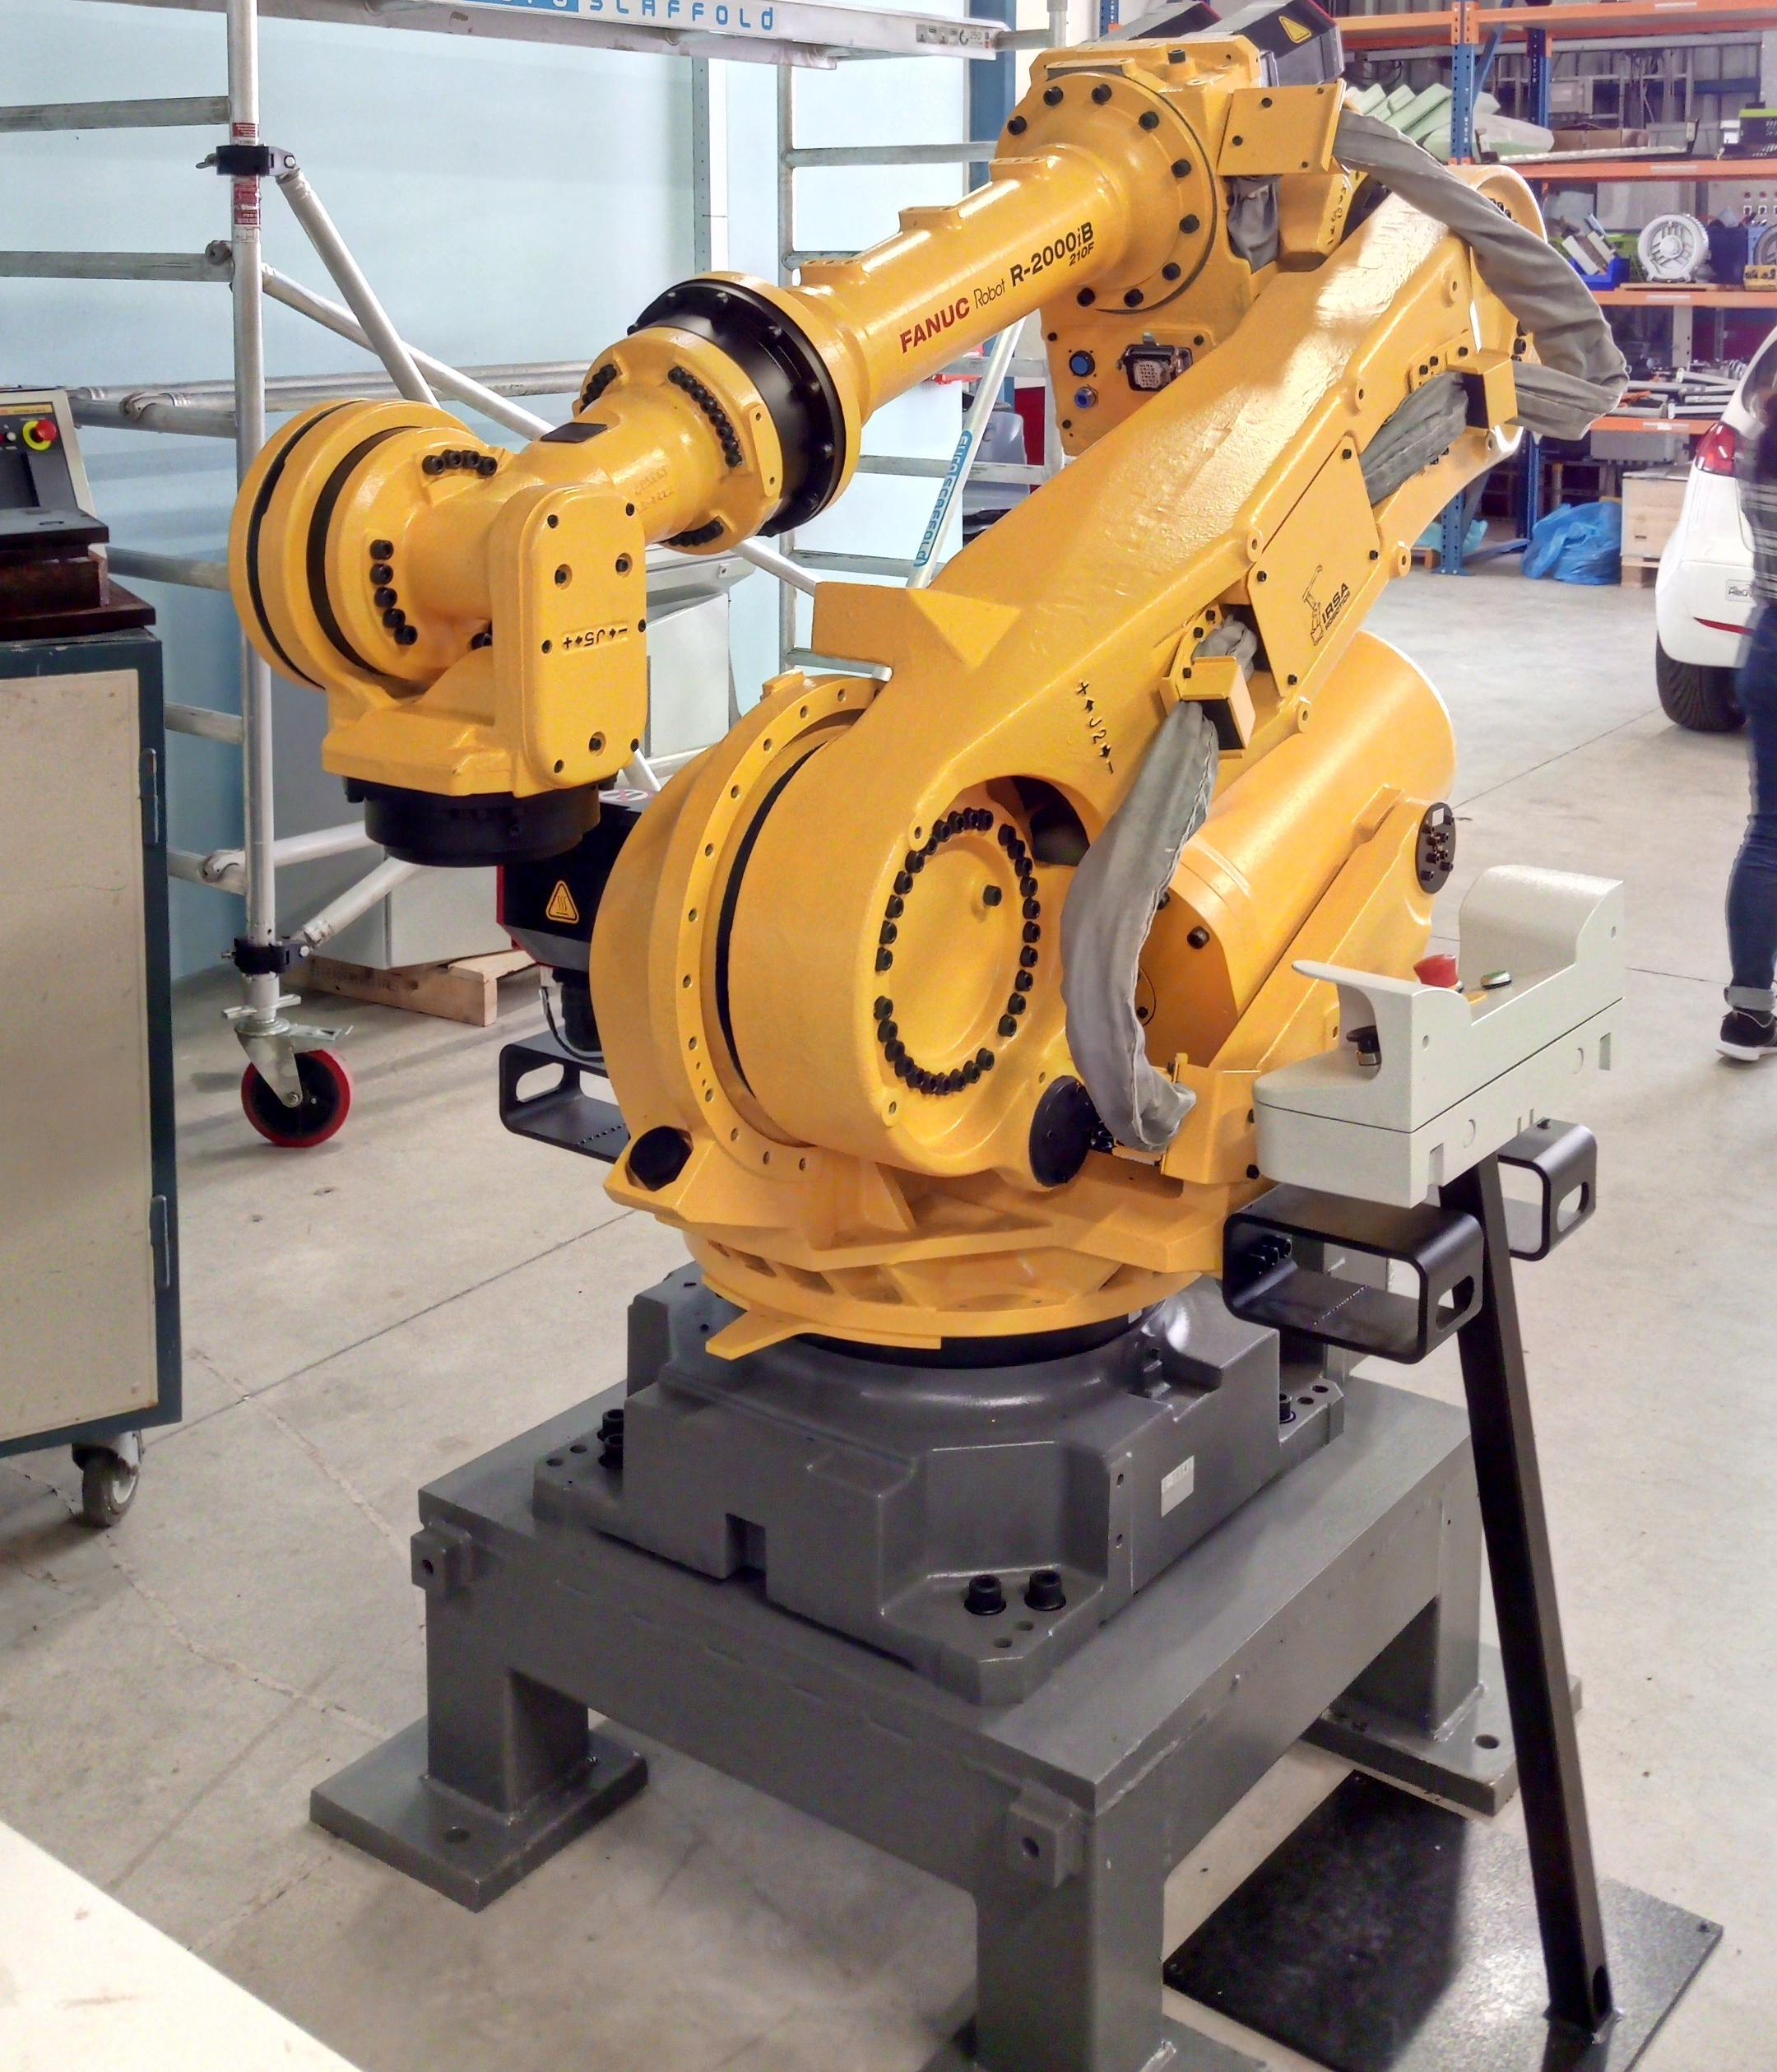
\includegraphics[
	width=0.6\linewidth,
	height=\paperheight,
	keepaspectratio,
	]{fanuc210_corner_cut}
	\caption{FANUC R-2000iC/210F 6-axis industrial robot arm}
	\label{fig:fanuc210}
\end{figure}





